\section{Isomorphismus}
\authors{Florian Weiser und Sebastian Leon Schmidt}
\subsection{Eigenschaften von Funktionen}
Oftmals ist das Umkehren einer Abbildung\footnote{Abbildungen sind eindeutige Zuordnungen zwischen zwei Mengen $D$ und $Z$. Jedem Element $x \in D$ wird durch die Abbildung $f$ genau ein Element $f(x) \in Z$ zugeordnet. Der Begriff Funktion wird meist synonym zu Abbildung benutzt.} nur mit Einschränkungen der Definitions- oder Wertemenge möglich. Im Folgenden sollen Eigenschaften definiert werden, welche bereits Rückschlüsse auf die Umkehrbarkeit von Abbildungen erlauben.
\subsubsection{Injektive Abbildungen}

\begin{df}Eine \wichtig{injektive Abbildung} (Injektion) ist eine Abbildung $f:A \rightarrow B$, durch die zu jedem Element $b \in B$ höchstens ein Element $a \in A$ mit $b=f(a)$ existiert.
\end{df}
Keine zwei verschiedenen Elemente der Definitionsmenge dürfen auf das selbe Element der Zielmenge abbilden. In \autoref{fig:iso01} ist eine injektive Abbildung zwischen den Mengen $A$ und $B$ visualisiert. Die Umkehrung einer injektiven Funktion ist im Bereich der tatsächlich angenommenen Werte möglich.

\begin{figure}[!h]
\centering
\begin{tikzpicture}[line width=1pt,>=latex]
\sffamily
\node (a1) {1};
\node[below=0.3cm of a1] (a2) {2};
\node[below=0.3cm of a2] (a3) {3};
\node[below=0.3cm of a3] (a4) {};

\node[right=3cm of a1] (b1) {a};
\node[below=0.3cm of b1] (b2) {b};
\node[below=0.3cm of b2] (b3) {c};
\node[below=0.3cm of b3] (b4) {d};

\node[shape=ellipse,inner sep=-3pt,draw=black,minimum size=1.8cm,fit={(a1) (a4)}] {};
\node[shape=ellipse,inner sep=-3pt,draw=black,minimum size=1.8cm,fit={(b1) (b4)}] {};

\node[below=0.7cm of a4,font=\color{black}\Large\bfseries] (a) {A};
\node[right = 3cm of a,font=\color{black}\Large\bfseries] (b) {B};

\draw[->,black] (a1) -- (b1);
\draw[->,black] (a2) -- (b2);
\draw[->,black] (a3) -- (b4);
%\draw[->,black] (a4.20) -- (b2.190);
\end{tikzpicture}
\caption{Illustration einer injektiven Abbildung}\label{fig:iso01}
\end{figure}

\subsubsection{Surjektive Abbildungen}
\begin{df}Eine \wichtig{surjektive Abbildung} (Surjektion) ist eine Abbildung $f : A \rightarrow B$, durch die jedes $b \in B$ mindestens ein Urbild in der Menge $A$ besitzt.\end{df}
\autoref{fig:iso02} veranschaulicht eine surjektive Abbildung von $A$ auf $B$.
Surjektive Abbildungen (Surjektionen) sind nicht notwendigerweise eindeutig umkehrbar, weil einige Elemente aus B mehrere Urbilder besitzen können.\\

\begin{figure}[!h]
\centering
\begin{tikzpicture}[line width=1pt,>=latex]
\sffamily
\node (a1) {1};
\node[below=0.3cm of a1] (a2) {2};
\node[below=0.3cm of a2] (a3) {3};
\node[below=0.3cm of a3] (a4) {4};

\node[right=3cm of a1] (b1) {a};
\node[below=0.3cm of b1] (b2) {b};
\node[below=0.3cm of b2] (b3) {c};
\node[below=0.3cm of b3] (b4) {};
\node[right=3cm of a4] (bl) {};

\node[shape=ellipse,inner sep=-3pt,draw=black,minimum size=1.8cm,fit={(a1) (a4)}] {};
\node[shape=ellipse,inner sep=-3pt,draw=black,minimum size=1.8cm,fit={(b1) (bl)}] {};

\node[below=0.7cm of a4,font=\color{black}\Large\bfseries] (a) {A};
\node[right = 3cm of a,font=\color{black}\Large\bfseries] (b) {B};

\draw[->,black] (a1) -- (b1.170);
\draw[->,black] (a2) -- (b2.175);
\draw[->,black] (a3) -- (b3.175);
\draw[->,black] (a4) -- (b3.190);
%\draw[->,black] (a4.20) -- (b2.190);
\end{tikzpicture}
\caption{Illustration einer surjektiven Abbildung}\label{fig:iso02}
\end{figure}

\subsubsection{Bijektive Abbildungen}
\begin{df}Eine \wichtig{bijektive Abbildung} (Bijektion) ist eine Abbildung $f : A \rightarrow B$, die sowohl injektiv als auch surjektiv ist.\end{df}

Zwischen der Definitionsmenge und Bildmenge einer bijektiven Funktion besteht eine Eins-zu-Eins-Beziehung. Jedem Element aus der Menge $A$ wird dabei exakt ein Element aus der Menge $B$ zugeordnet und alle Elemente aus $B$ besitzen genau ein Urbild in A. Dieses Verhältnis ist in \autoref{fig:iso03} veranschaulicht. Man spricht von einer eineindeutigen Zuordnung.
Beispielsweise ist die Funktion $g (x) = x$ bijektiv im Bereich der reellen Zahlen.
Die Umkehrabbildung $f^{-1} : Y \rightarrow X$ einer bijektiven Funktion f mit $y \mapsto f^{-1}(y)$ kann ohne Einschränkungen gebildet werden.

\begin{figure}[!h]
\centering
\begin{tikzpicture}[line width=1pt,>=latex]
\sffamily
\node (a1) {1};
\node[below=0.3cm of a1] (a2) {2};
\node[below=0.3cm of a2] (a3) {3};
\node[below=0.3cm of a3] (a4) {4};

\node[right=3cm of a1] (b1) {a};
\node[below=0.3cm of b1] (b2) {b};
\node[below=0.3cm of b2] (b3) {c};
\node[below=0.3cm of b3] (b4) {d};
\node[right=3cm of a4] (bl) {};

\node[shape=ellipse,inner sep=-3pt,draw=black,minimum size=1.8cm,fit={(a1) (a4)}] {};
\node[shape=ellipse,inner sep=-3pt,draw=black,minimum size=1.8cm,fit={(b1) (bl)}] {};

\node[below=0.7cm of a4,font=\color{black}\Large\bfseries] (a) {A};
\node[right = 3cm of a,font=\color{black}\Large\bfseries] (b) {B};

\draw[->,black] (a1) -- (b1.170);
\draw[->,black] (a2) -- (b2.175);
\draw[->,black] (a3) -- (b3.175);
\draw[->,black] (a4) -- (b4.190);
%\draw[->,black] (a4.20) -- (b2.190);
\end{tikzpicture}
\caption{Illustration einer bijektiven Abbildung}\label{fig:iso03}
\end{figure}

\subsection{Isomorphismus}
\begin{df}Eine Abbildung $f : A \rightarrow B$ ist ein \wichtig{Isomorphismus}, wenn sie bijektiv und strukturerhaltend ist.\end{df}
%Eine Abbildung $f : A \rightarrow B$ ist ein \wichtig{Isomorphismus}, wenn sie eine Abbildung $g : B \rightarrow A$ existiert, sodass für alle $a \in A$, $b \in B$ gilt: $g(f(a)) = a$ und $f(g(b)) = b$.
%Im Gegensatz zur Bijektivität ist ein Isomorphismus nicht notwendigerweise eine Abbildung von Mengen, sondern die abgebildeten Objekte können eine zusätzliche Struktur besitzen können.
So ist etwa die Abbildung $h$ von $\mathbb{N}_0$ auf $\mathbb{Z}$ mit $h : n \mapsto (-1)\textsuperscript{n}\lceil\frac{n}{2}\rceil$ bijektiv, aber kein Isomorphismus, da die Struktur der Addition von Elementen nicht erhalten bleibt und zum Beispiel $h(2 + 3) \neq h(2) + h(3)$.

\subsection{Exkurs: Homotope Abbildungen}
\begin{df}
Sei $I$ das Einheitsintervall $[0, 1]$ und seien $f, g: X \rightarrow Y$ zwei stetige Abbildungen zwischen den topologischen Räumen $X$ und $Y$. Eine \wichtig{Homotopie} ist eine stetige Abbildung $H : X \times I \rightarrow Y$, welche die Eigenschaften
\begin{equation}
H(x, 0) = f(x)
\end{equation}
und
\begin{equation}
H(x, 1) = g(x)
\end{equation}
erfüllt.
\end{df}
Die Homotopie $H$ kann sich als Verformung einer Abbildung in eine andere vorgestellt werden.\\
Zwei Abbildungen sind homotop zueinander, wenn eine Homotopie für sie existiert.\\
\wichtig{Beispiel:} Sei $S^1$ eine 1-dimensionale Sphäre\footnote{Eine 1-dimensionale Sphäre wird auch als Kreislinie bezeichnet} und $T^2$ ein 2-dimensionaler Torus. In \autoref{fig:hlg} sind die Abbildungen $a, b, c: S^1 \rightarrow T^2$ im topologischen Raum des Torus eingezeichnet. Die Abbildungen $a$ und $c$ sind homotop zueinander, weil sich die eine Abbildung durch Verformung der anderen auf der Oberfläche des Torus erreichen lässt. Da die eingezeichneten Abbildungen außer $b$ homotop zu einem Punkt sind, gibt es keine Homotopie zwischen $b$ und einer der beiden anderen Abbildung.

\begin{figure}[!h]
%\makebox[\textwidth][c]{\includegraphics[width=1.2\textwidth]{Torus}}
%\centerfloat
%\includegraphics{Torus}
\includegraphics[scale=0.67]{img/Torus}
%\includesvg{Torus}
\caption{Kreislinien a, b und c auf der Oberfläche eines Torus (Bildnachweis: https://en.wikipedia.org/wiki/File:Toruscycles1.svg von Steelpillow; Lizenz: Creative Commons Attribution-Share Alike 4.0i; Kreislinie a neu platziert)}\label{fig:hlg}
\end{figure}

%Als Homotopie wird eine stetige Deformation zweier Abbildungen $f$ und $g$ zwischen den topologischen Räumen $X$ und $Y$ bezeichnet. Für die stetige Abbildung H $X \times [0, 1]$,  $\rightarrow$ Y mit H(x, 0) = f(x) und H(x, 1) = g(x) gibt. Man kann sich die Abbildung H auch als Verformung einer Abbildung in eine andere vorstellen. Neben der Eigenschaft von Abbildungen wird H ebenfalls als Homotopie bezeichnet.\\
%Beispiel: Sei S1 eine 1-dimensionale Sphäre  und T2 ein Torus. Zwei nach der Vorschrift fi: S1 $\rightarrow$ T2 gebildete Abbildungen sind im topologischen Raum eines Torus in der Grafik blau und rot gekennzeichnet. Durch Verformung der einen Abbildung auf der Oberfläche des Tubus kann man die andere Abbildung nicht erhalten, deshalb sind sie nicht homotop.

\subsection{Elementlose Isomorphismusdefinition}
Der Exkurs zu homotopen Abbildungen soll als Motivation für eine elementlose Definition von Isomorphismus dienen. 
\begin{df}
Eine Abbildung $f : A \rightarrow B$ ist ein Isomorphismus, wenn es eine Abbildung $g : B \rightarrow A$ gibt, sodass $g \circ f = id_{A}$ und $f \circ g = id_{B}$.
\end{df}

\subsection{Isomorphe Graphen}
Die elementlose Definition von Isomorphismus kann auch auf Graphen angewandt werden.
\begin{df} Sei $p$ eine bijektive Abbildung $p : V \rightarrow V'$ mit $G = (V,E)$ und $G' = (V',E')$. Die Abbildung $p$ ist ein \wichtig{Isomorphismus}, falls $(u, v) \in E \Leftrightarrow (p(u), p(v)) \in E'$ gilt.
\end{df}
Zwei isomorphe Graphen müssen die gleiche Knoten- und Kantenmenge besitzen. Sie können so gezeichnet werden, dass sie identisch aussehen. Für den Nachweis eines Isomorphismus ist es oftmals nützlich, den Knoten Nummern zuzuordnen und zu prüfen, ob die von einem Knoten ausgehenden Kanten in beiden Graphen übereinstimmen. \autoref{fig:iso} zeigt zwei isomorphe Graphen mit enstprechend nummerierten Knoten.
\begin{figure}
\centering
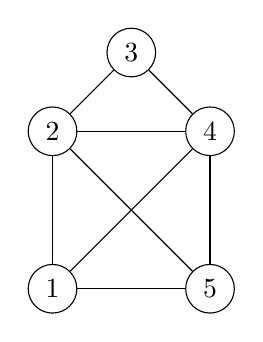
\begin{tikzpicture}
\node[draw, circle](a) at (1,0){1};
\node[draw, circle](b) at (1,2){2};
\node[draw, circle](c) at (2,3){3};
\node[draw, circle](d) at (3,2){4};
\node[draw, circle](e) at (3,0){5};
\draw (a) -- (b);
\draw (a) -- (d);
\draw (b) -- (d);
\draw (b) -- (e);
\draw (c) -- (b);
\draw (c) -- (d);
\draw (d) -- (e);
\draw (a) -- (e);
\end{tikzpicture}
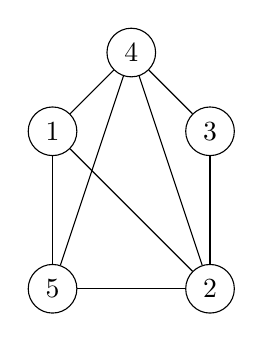
\begin{tikzpicture}
\node[draw, circle](a) at (4,2){1};
\node[draw, circle](b) at (6,0){2};
\node[draw, circle](c) at (6,2){3};
\node[draw, circle](d) at (5,3){4};
\node[draw, circle](e) at (4,0){5};
\draw (a) -- (b);
\draw (a) -- (d);
\draw (b) -- (d);
\draw (b) -- (e);
\draw (c) -- (b);
\draw (c) -- (d);
\draw (d) -- (e);
\draw (a) -- (e);
\end{tikzpicture}
\caption{Isomorphe Graphen}\label{fig:iso}
\end{figure}
